
\PassOptionsToPackage{table}{xcolor}

\documentclass[sigconf%
,natbib=true%
]{acmart}

\graphicspath{{figures/}}

\AtBeginDocument{%
  \providecommand\BibTeX{{%
    \normalfont B\kern-0.5em{\scshape i\kern-0.25em b}\kern-0.8em\TeX}}}

\copyrightyear{2020}
\acmYear{2020}
\setcopyright{rightsretained}
\acmConference[VINCI 2020]{The 13th International Symposium on Visual
	Information Communication and Interaction}{December 8--10,
	2020}{Eindhoven, Netherlands}
\acmBooktitle{The 13th International Symposium on Visual Information
	Communication and Interaction (VINCI 2020), December 8--10, 2020,
	Eindhoven, Netherlands}\acmDOI{10.1145/3430036.3430041}
\acmISBN{978-1-4503-8750-7/20/12}

\acmSubmissionID{5}



\usepackage{microtype}
\usepackage{tabularx}
\usepackage{enumitem}
\usepackage{csquotes}
\usepackage{tikz}
\usepackage{pifont}
\usepackage{amsmath}
\usepackage{calc}
\usepackage{booktabs}
\usepackage{ifthen}
\usepackage{wrapfig}
\usetikzlibrary{patterns}
\usetikzlibrary{matrix}
\usetikzlibrary{arrows}
\usetikzlibrary{fit}
\usetikzlibrary{calc}
\usetikzlibrary{positioning}

\usepackage{multirow}
\usepackage{makecell}

\newcommand*\rot{\rotatebox{90}}
\newcommand*\rotc{\rotatebox[origin=rb]{270}}
\newcommand*\OK{$\bullet$}
\newcommand*\UP{\ding{218}}
\newcommand*\DOWN{\ding{216}}

\newcommand*\PARTIAL{$\circ$}
\newcommand*\NA{\cellcolor{gray!40}}
\newcommand*\UNKNOWN{--}

\definecolor{tablelightgray}{gray}{0.8}
\newcommand*\tls{\color{tablelightgray}\vrule width 0.4pt} %

\newcommand{\mc}[2]{\multicolumn{#1}{c|}{\makecell{#2}}} %
\newcommand{\mct}[2]{\mc{#1}{\tiny #2}} %
\newcommand{\rott}[1]{\rot{\tiny #1}}

\newlength{\largestheaderlength}%

\definecolor{applegreen}{rgb}{0.55, 0.71, 0.0}

\newcommand{\pprelim}[1]{\color[rgb]{0.5,0.5,0.5}#1}
\newcommand{\pfeedback}[1]{\color[rgb]{0.8,0.1,0.1}#1}
\newcommand{\previsit}[1]{\color[rgb]{0.1,0.3,0.8}#1}
\newcommand{\pfinal}[1]{\color{black}#1}

\makeatletter
\newcommand\queryfont{%
	\f@size
}
\makeatother

\newcommand{\addcite}{~\cite{?}}

\newcommand*\Ts {$\mathcal{T}_{\mathrm{S}}$}
\newcommand*\Tc {$\mathcal{T}_{\mathrm{C}}$}
\newcommand*\Tie{$\mathcal{T}_{\mathrm{IE}}$}
\newcommand*\Tmt{$\mathcal{T}_{\mathrm{MT}}$}
\newcommand*\Th{$\mathcal{H}$}

\usepackage{localreference}

\usepackage{enumitem}
\setlist[description]{%
    font        = \normalfont\itshape\space,%
    leftmargin  = 3.0\parindent,%
    labelindent = \parindent}

\begin{document}

\title{Survey of Treemap Layout Algorithms}

\author{Willy Scheibel}
\orcid{0000-0002-7885-9857}
\email{willy.scheibel@hpi.de}
\affiliation{%
  \institution{Hasso Plattner Institute,\\Faculty of Digital Engineering, University of Potsdam, Germany}
}
\author{Daniel Limberger}
\orcid{0000-0002-9111-4809}
\email{daniel.limberger@hpi.de}
\affiliation{%
  \institution{Hasso Plattner Institute,\\Faculty of Digital Engineering, University of Potsdam, Germany}
}
\author{J{\"u}rgen D{\"o}llner}
\email{juergen.doellner@hpi.de}
\affiliation{%
  \institution{Hasso Plattner Institute,\\Faculty of Digital Engineering, University of Potsdam, Germany}
}

\renewcommand{\shortauthors}{W.~Scheibel, D.~Limberger, J.~D{\"o}llner}

\begin{abstract}
    This paper provides an overview of published treemap layout algorithms from 1991 to 2019 that were used for information visualization and computational geometry.
    First, a terminology is outlined for the precise communication of tree-structured data and layouting processes.
    Second, an overview and classification of layout algorithms is presented and application areas are discussed.
    Third, the use-case-specific adaption process is outlined and discussed.
    This overview targets practitioners and researchers by providing a starting point for own research, visualization design, and applications.
\end{abstract}

\begin{CCSXML}
    <ccs2012>
    <concept>
    <concept_id>10003120.10003145.10003146.10010889</concept_id>
    <concept_desc>Human-centered computing~Treemaps</concept_desc>
    <concept_significance>500</concept_significance>
    </concept>
    <concept>
    <concept_id>10003120.10003145.10011770</concept_id>
    <concept_desc>Human-centered computing~Visualization design and evaluation methods</concept_desc>
    <concept_significance>500</concept_significance>
    </concept>
    </ccs2012>
\end{CCSXML}

\ccsdesc[500]{Human-centered computing~Treemaps}
\ccsdesc[500]{Human-centered computing~Visualization design and evaluation methods}

\keywords{Treemap Layout Algorithms, Tree Spatialization, Graph Drawing}

\maketitle
\section{Introduction}
For much of today's tree-structured data---either inherent or otherwise supplemented---the family of treemap visualization techniques provide a versatile and well established way for visualization~\cite{mcnabb2017-surveyofsurveys}.
As such, the domains of software visualization~\cite{limberger2019-softwaremap} (Figure~\ref{fig:teaser}), demographics~\cite{jern2009-regionalstatistics}, biology and medicine~\cite{chazard2006-medicaldata}, and business data~\cite{roberts2018-businessdata} deal with complex, tree-structured datasets, and have a growing need for visualization.
Since the introduction of treemaps~\cite{johnson1991-spacefilling}, related research is present at conferences and in journals every year, publishing advances in data processing, layouting techniques, visual variable mapping and encoding, and applications.
\par
Eventually, this led to a large and even growing number of treemap layout algorithms.
These number of algorithms and visualization techniques were consolidated in design spaces and surveys before.
As such, Schulz~et~al. proposed both a design space for 3D treemaps~\cite{schulz2007-poster} and an extension to this design space to cover implicit tree visualizations more generally~\cite{schulz2011-implicit}.
A visual survey on tree visualization techniques in general is published at \href{treevis.net}{https://treevis.net}~\cite{schulz2011-treevis}.
More specifically with focus on treemaps, Shneiderman provides tool-centric view on treemap visualization techniques \cite{shneiderman2009-treemaps}.
All of these publications focus on the visualization technique and the visual encoding.
Focusing more on the layout algorithms, Baudel and Broeksema proposed a design space of sequential, space-filling layouts \cite{baudel2012-designspace}, that was extended by Schulz~et~al. for general rooted tree drawings \cite{schulz2013-generativelayout}.
\par
On one hand, this availability leave visualization designers to question which algorithm is suited for their intend.
On the other hand, the selection of an appropriate algorithm may be driven by technical decisions.
For example, the size of the dataset and the data that should be visually encoded needs to be considered as well.
As the distinction between treemap visualization techniques and general tree visualization techniques has been published and is open for discussion~\cite{scheibel2020-treemaptaxonomy}, this survey focuses on layout algorithms that employ \enquote{the property of containment}~\cite{johnson1993-categorical} exclusively, i.e., containment treemaps \Tc{}.
As such, we consider algorithms that
\begin{itemize}
    \item map a rooted tree into a $k$D layout space ($k \in \mathbb{N}^*$),
    \item account for multiple attributes and additional relations, and
    \item distribute child nodes \emph{within} their parents' extent.
\end{itemize}
\par
This paper presents a review of said algorithms by (1) recapitulating and consolidating basic terminology used, (2) presenting a classification of their characteristics, and (3) providing guidance for the choice of algorithm for applications of treemaps.
Starting with the initial publication of treemaps in 1991, we considered 81 treemap layout algorithms published in conference proceedings and journal articles of major publishers---IEEE, ACM, Springer, EG, Elsevier, and SciTePress---as well as selected doctoral theses in the years from 1991 to 2019.
\begin{figure}[b]%
	\centering%
	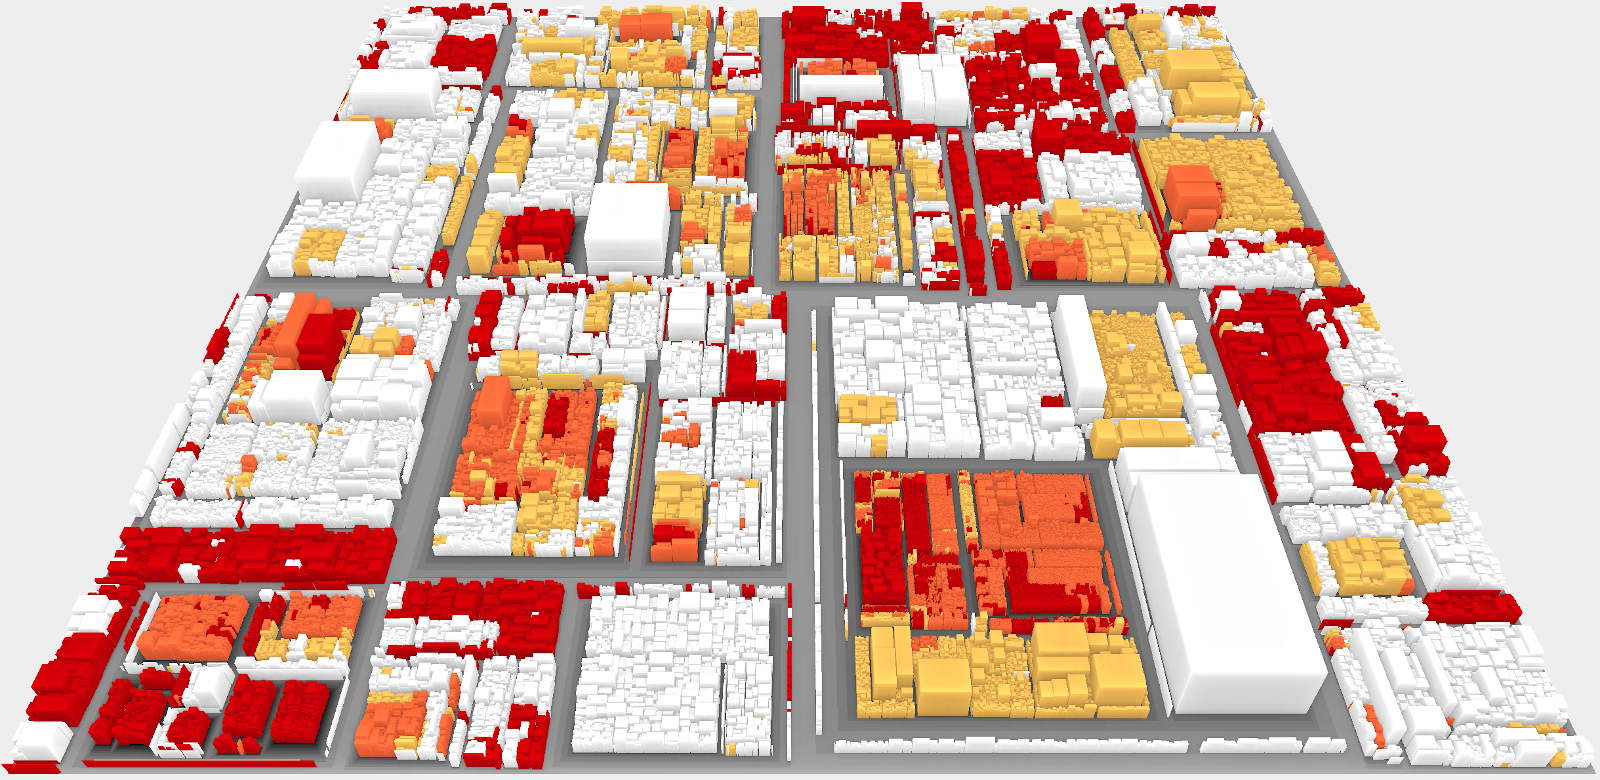
\includegraphics[width=1.0\linewidth]{figures/teaser.png}%
	\caption{Example 2.5D treemap visualization of the source code files of the Firefox software project with 109\,000 nodes using the Hilbert treemap layout algorithm and recursive nested depiction of child nodes.}%
	\label{fig:teaser}
\end{figure}%
\par
The remainder of this paper is structured as follows.
Section~2 recapitulates terminology used for tree-structured data and treemap layouting techniques.
Section~3 reviews available layout algorithms for treemaps.
Section~4 discusses adaptation and layout postprocessing.
Section~5 concludes this paper.

\section{Treemap Termini}

Depictions of tree-structured data are subject to research for at least a century~\cite{gannett1903-census}.
The language used to discuss and communicate their making, intent, and effectiveness has changed and most likely will continue to change.
Although the purpose of this section is to facilitate unambiguous and precise communication, we are aware of the general ambiguity of language and different approaches to modeling and communication. %
Nevertheless, we reiterate common terms for \emph{tree structure} and \emph{spatialization} using notions of graph theory~\cite{diestel2010-graphtheory} and visualization theory.
As a general case, a tree-structured dataset can be modeled as a graph built up by vertices (data points) and at least one relationship among the vertices represented by edges.
\paragraph{\textbf{Tree Structure Termini}}
For a dataset to be suitable for treemapping, the expected structure---the topology---of the nodes and edges is expected to be a rooted tree. Often, we find the term \emph{hierarchy} to be used synonymously, but we suggest to strictly distinguish. As an additional special case, a dataset with forest structure can be used for treemapping by employing a virtual root node.
\begin{description}
    \item[Hierarchy.] A special type of a graph with the characteristics that there is one type of directed relation (and, thus, one type of directed edges) encoding a parent-child relationship with no circles (synonym: directed, acyclic graph).
    \item[Tree.] A special type of a hierarchy with the main characteristic that the hierarchy is \emph{arborescent}, i.e., it has a single vertex with no parent relationship, each other vertex has exactly one \emph{parent} vertex.%
	\item[Forest.] A special type of hierarchy that represents a set of trees, i.e., there may be multiple vertices with no parent relationship.
	\item[Topology.] The relationships between vertices, i.e., the set of edges of a graph.
\end{description}
\begin{figure}[t]%
	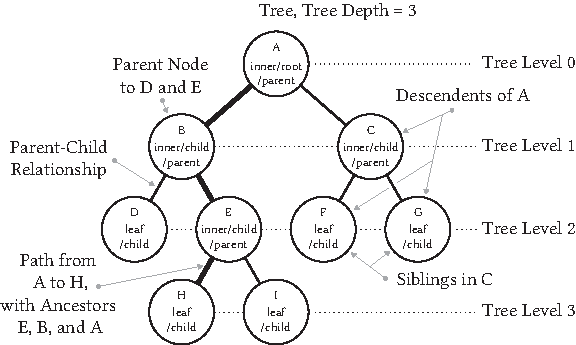
\includegraphics[width=\linewidth]{tree-taxonomy}
	\caption{A tree-structure depiction with annotated terms.}
	\label{fig:treetermini}
\end{figure}
With respect to a tree-structured dataset, there are additional termini to precisely denote characteristics, assumptions, and algorithms for treemap visualizations (\autoref{fig:treetermini}):
\begin{description}
	\item[Node.] The representation of a data point in the semantics of a tree in information visualization (i.e., a vertex in graph theory).
	\item[Relation.] The representation of a relation between two nodes (i.e., an edge in graph theory).
	\item[Parent-Child Relationship.] A directed relation connecting two nodes, in which context one node has the \emph{parent} role and the other has the \emph{child} role.
	\item[Parent Node / Inner Node.] A node that has child nodes, i.e., it has one or more relationships with other nodes where the node itself is \emph{parent}.
	\item[Root Node] A node of a tree that has no parent node. For actual trees there is only a single node per tree, for forests there is one for each tree of the forest.
	\item[Child Node.] A node that has a parent node, i.e., it has a relationship with another node where the node itself is \emph{child}. 
	\item[Leaf Node.] A node without associated child nodes.
\end{description}

\noindent For such a tree, additional properties and concepts can be applied that are used when deriving treemaps:
\begin{description}
	\item[Path.] The shortest list of nodes that connects two nodes using the parent-child relationship. Thereby, the first node is the source node, the last node is the target node and each two adjacent nodes in the list are connected through a parent-child relationship.
	\item[Ancestors.] The set of nodes on the path from the parent node to the root node.
	\item[Descendants.] The recursively collected set of all child nodes and their child nodes starting at one or more nodes.
	\item[Siblings.] The set of child nodes with the same parent node.
	\item[Node Depth.] The length of the path to the root node excluding the node itself.
	\item[Tree Depth.] The maximum node depth across all nodes of a tree.
	\item[Tree Level.] One level of a tree is the set of nodes with the same node depth. This is sometimes called a tree slice.
\end{description}
While the tree is the main data structure to derive treemap visualizations, actual datasets may be augmented with other structural information.
To this end, a dataset that is used for treemaps is not required to have one single type of edges to make it a tree, but that there is one type of edge that allows for an arborescent view on the graph.
Thus, some algorithms and techniques make use of the following concepts:
\begin{description}
	\item[Compound Tree.] A tree with additional relations between nodes that are not used as parent-child relationships.
	\item[Neighborhood Information.] The availability of additional relations between sibling nodes that should be considered during node layouting and visualization.
\end{description}
Thereby, neighborhood information may be relevant for treemap layouting, but general additional relationships are more prominently used for superimposed edge visualization \cite{holten2006-edgebundles}.

\begin{figure}[t]
    \definecolor{gray-1}{RGB}{144,144,144}
    \definecolor{gray-2}{RGB}{160,160,160}
    \definecolor{gray-3}{RGB}{176,176,176}
    \definecolor{gray-4}{RGB}{192,192,192}
    \newcommand{\newrect}[3]{%
    	\node[fit={(#2)($(#2)+(#3)$)}] (#1) {};%
    }
    \newcommand{\newlocalrect}[6]{%
    	\node[fit={(#2:#3,#4)($(#2:#3+#5,#4+#6)$)}] (#1) {};%
    }
    \newcommand{\localrect}[5]{
    	(#1:#2,#3) rectangle (#1:#2+#4,#3+#5)
    }
    \centering
    \begin{tikzpicture}[inner sep=0pt, outer sep=0pt]
        \newrect{splitting-layout}{0cm,0cm}{4.0cm,4.0cm};
		\node[above=0.15cm of splitting-layout.north,text depth=0pt] {\footnotesize Splitting Layout};
		\newlocalrect{splitting-layout-a}{splitting-layout}{0.0}{0.0}{0.55}{0.5};
		\newlocalrect{splitting-layout-b}{splitting-layout}{0.0}{0.5}{0.45}{0.5};
		\newlocalrect{splitting-layout-c}{splitting-layout}{0.45}{0.5}{0.55}{0.5};
		\newlocalrect{splitting-layout-d}{splitting-layout}{0.55}{0.0}{0.45}{0.5};
		\draw[fill=gray-1] \localrect{splitting-layout-a}{0.0}{0.0}{1.0}{1.0};
		\draw[fill=gray-2] \localrect{splitting-layout-b}{0.0}{0.0}{1.0}{1.0};
		\draw[fill=gray-3] \localrect{splitting-layout-c}{0.0}{0.0}{1.0}{1.0};
		\draw[fill=gray-4] \localrect{splitting-layout-d}{0.0}{0.0}{1.0}{1.0};
		
        \newrect{packing-layout}{4.5cm,0cm}{4.0cm,4.0cm};
		\node[above=0.15cm of packing-layout.north,text depth=0pt] {\footnotesize Packing Layout};
		\newlocalrect{packing-layout-a}{packing-layout}{0.0}{0.1}{0.55}{0.4};
		\newlocalrect{packing-layout-b}{packing-layout}{0.1}{0.5}{0.35}{0.5};
		\newlocalrect{packing-layout-c}{packing-layout}{0.45}{0.5}{0.55}{0.4};
		\newlocalrect{packing-layout-d}{packing-layout}{0.6}{0.0}{0.35}{0.5};
		\draw[] \localrect{packing-layout}{0.0}{0.0}{1.0}{1.0};
		\draw[fill=gray-1] \localrect{packing-layout-a}{0.0}{0.0}{1.0}{1.0};
		\draw[fill=gray-2] \localrect{packing-layout-b}{0.0}{0.0}{1.0}{1.0};
		\draw[fill=gray-3] \localrect{packing-layout-c}{0.0}{0.0}{1.0}{1.0};
		\draw[fill=gray-4] \localrect{packing-layout-d}{0.0}{0.0}{1.0}{1.0};
    \end{tikzpicture}
    \caption{Conceptual display of splitting vs. packing layouts. Splitting layout algorithms utilize the whole space of a layout element for subdivision whereas packing layouts usually contain white space.}
    \label{fig:layouttermini}
\end{figure}

\paragraph{\textbf{Spatialization Termini}}
The layout of a treemap is one of its unique features.
Hence, the layouting process and its characteristics have specific termini (\autoref{fig:layouttermini}).
In graph theory, the layouting process is also known as \emph{graph drawing}~\cite{eppstein2012-areauniversal}.
\begin{description}
	\item[Treemap Layout.] A set of polytopes within the dimensionality of the reference space, e.g., polygons for 2-dimensional layouts, that are associated with the nodes of a tree. The polytopes adhere to the property of containment.
	\item[Treemap Layout Element.] A single polytope of a treemap layout, usually associated with the node it represents.
	\item[Treemap Layout Algorithm.] An algorithm that maps tree-struc\-tured data to a treemap layout.
	\item[Space-filling.] This property indicates that a layout algorithm generates layouts where the allocated space is fully used.
	\item[Geo-dependent.] A layout algorithm is geo-dependent if the generated layouts adhere to given geo-spatial constraints, e.g., geo-referenced neighbors~\cite{slingsby2009-configuring,buchin2011-adjacency}. A synonym for this characteristic is \emph{spatially dependent}.
	\item[Packing Approach.] A layout algorithm is a packing algorithm if the layout of an inner node is derived from the layout of its child nodes~\cite{schulz2011-implicit}.
	\item[Splitting Approach.] A layout algorithm is a splitting algorithm if the layout of a node is derived from the layout of its parent node~\cite{schulz2011-implicit}.
	This process is also called dissection~\cite{namagochi2007-dissecting}.
\end{description}

\section{Treemap Layout Algorithms}
Layouting is the mapping of a node into a reference space which typically is one-dimensional, two-dimensional or three-dimensional.
This layouting is considered a recursive algorithm, whereby a treemap algorithm usually defines the layout for one level of the tree.
For an algorithm to count as treemap layout algorithm, we require it to represent the parent-child relationship between nodes by containment, i.e., to layout a child node within the layout of the parent node. %
Besides the parent-child relationship, other information such as a size attribute or neighborhood information among child nodes can be used as well.

\subsection{Definition of a Treemap Layout Algorithm}
The task to identify a treemap layout algorithm depends on two definitions. 
First, it must be determinable if a resulting layout is in fact a treemap layout, i.e., if it adheres to a definition of a treemap layout.
In order to provide a more specific yet minimal working definition, we consider a treemap layout as follows:
\begin{definition}{Treemap Layout} \\%\vspace{0.25\baselineskip}\\
	\label{def:treemaplayout}%
	A treemap layout associates a treemap layout element for each node of a tree.
	For all layout elements and their associated nodes, the following conditions must be met.
	\begin{enumerate}
		\item[(i)] Layout elements of any sibling nodes $p$ and $q$ must not overlap.
		\item[(ii)] If $p$ is ancestor of $q$, then the layout element of $q$ is fully enclosed by layout element of $p$.
	\end{enumerate}
\end{definition}
This ensures that the layout element of a child node is located within the layout element of its parent node and does not overlap with any sibling layout element.
With respect to Definition \ref{def:treemaplayout}, a treemap layout algorithm is an algorithm or function that maps a tree to a treemap layout.
This results in a large set of algorithms to be considered treemap layout algorithms.
In this paper, we focus on algorithms that derive such a layout from a rooted tree, while not using another treemap layout for the same tree as additional input.
\begin{definition}{Treemap Layout Algorithm} \\%\vspace{0.25\baselineskip}\\
	\label{def:treemaplayoutalgorithm}%
	An algorithm that performs a graph drawing on a tree and results in an association of tree nodes to layout elements.
	The second required property is that this algorithm does not take another treemap layout for the same input tree as additional input.
\end{definition}
Those algorithms, that use such a pre-existing treemap layout for the rooted tree, we call \emph{treemap layout postprocessing algorithms}.

\subsection{Layout Algorithm Characteristics}
With respect to the scope of this paper, we assess the layout algorithms by a small set of properties.
As first classification, \enquote{one can discern two major layout methodologies: \emph{subdivision} and \emph{packing}}~\cite{schulz2011-implicit}.
The basic approach for \emph{packing layouts} is the arrangement of the polytopes of all child nodes in proximity and defining an enclosing polytope as own layout.
This approach is then applied recursively from leaf nodes to the root node.
Regarding \emph{splitting layouts}, the basic approach is to define a polytope for the root node and perform a dissection on its layout for its child nodes, recursing down the tree.
This basically means that all algorithms that perform a packing or subdivision of lines, areas, volumes, or even higher-dimensional shapes, are suitable for recursion and thus, for treemap layouting.
Next to the layouting methodology, the dimensionality of the reference space for the layout is important, as it mainly restricts further visual variable mapping.
For example, a 2.5D treemap, where the layout provides the space for 3D polytopes and the height of the polytopes is intended for height mapping, requires the layout to be one-dimensional or two-dimensional.

Another set of properties is the type of additional data an algorithm uses when layouting a tree.
Here, we use four different types of input data: (1) to use node weights for layout sizes, (2) to use neighborhood information to place layouts aside, (3) to use a similarity measure to place layouts in vicinity, and (4) to use another treemap layout of another rooted tree as starting point.
Especially for the node weights, we assess if the algorithms use the weight values to scale the sizes of leaf nodes. Typically, the size of parent nodes is adjusted to the spatial consumption of the child nodes.
Next, the type of shapes an algorithm chooses for the resulting layout is often a key filter of choice.
Typically, the class of shapes resembles either round shapes (points, circles, ellipsoids), axis-aligned shapes (lines, rectangles, boxes), other convex shapes (triangles, polygons, polytopes), and general non-convex shapes.
\par
There are more characteristics of treemap layout algorithms that may help to discern them and select one, e.g., the distinction between slicable and non-slicable layouts~\cite{young2003-twinbinary}, or the algorithms' run-time complexity (note that \enquote{the generic problem of creating such layouts fall in the category of NP-hard problems}~\cite{baudel2012-designspace}).
However, slicable layouts as well as run-time complexity in general are scarcely discussed within the community of information visualization. For this paper, we deliberately omitted additional, external assessment of these layouts.
Summarizing, we assess treemap layout algorithms along the following, non-exhaustive axes:
\begin{itemize}
    \item Iteration approach: packing and splitting
    \item Additional attributes: weight, neighborhood-preserving, and similarity
    \item Layout shape: circular, rectangular, convex, and non-convex
    \item Reference space dimensionality: 1D, 2D, and 3D
\end{itemize}

\subsection{Algorithm Overview}
The collected treemap layout algorithms (as defined with Definition~\ref{def:treemaplayoutalgorithm}) and their properties are provided in \autoref{table:layoutalgorithmoverview}.
This introduction and classification is broadly categorized by
(1) topology-focused layouts,
(2) list-focused layout algorithms,
(3) rectangular Splitting layouts,
(4) rectangular Packing layouts,
(5) rectangular 3D layouts,
(6) circular layouts,
(7) polygonal layouts,
(8) similarity-Map layouts,
(9) cartograms, and
(10) generalized layout algorithms.
For a broader perspective, we briefly include layout algorithms used outside of information visualization, too.

\begin{table}[tp]%
	\centering%
	\scriptsize%
	\noindent%
	\renewcommand{\arraystretch}{0.99}%
	\rowcolors{1}{white}{gray!15}%
	\setlength{\tabcolsep}{2.4pt}%
	\caption{%
		List of treemap layout algorithms (as defined with Definition~\ref{def:treemaplayoutalgorithm}) in approximated publication order.
		\vspace{-0.7\baselineskip}
	}%
	\label{table:layoutalgorithmoverview}%
	\begin{tabular}%
		{rc|ll|lll|llll|lll|}
		\rot{Algorithm} & \rot{Year} & \rot{Packing} & \rot{Splitting} & \rot{Weight} & \rot{Neighborhood} & \rot{Similarity} & \rot{Circular} & \rot{Rectangular} & \rot{Convex} & \rot{Non-Convex} & \rot{1D} & \rot{2D} & \rot{3D}\\
		\hline%
        Slice-and-Dice \cite{johnson1991-spacefilling} & 1991 &  & \OK & \OK &  &  &  & \OK &  &  &  & \OK & \\
        1-D Partitioning \cite{johnson1993-categorical} & 1993 &  & \OK & \OK &  &  &  & \OK &  &  & \OK &  & \\
        n-D Partitioning \cite{johnson1993-categorical} & 1993 &  & \OK & \OK &  &  &  & \OK &  &  & \OK & \OK & \OK\\
        Information Cube \cite{rekimoto1993-transparency} & 1993 &  & \OK & \OK &  &  &  & \OK &  &  &  &  & \OK\\
        Interactive Dynamic Map \cite{zizi1994-hyperdocuments} & 1994 &  & \OK & \OK &  &  &  & \OK &  &  &  & \OK & \\
        Guillotineable Bin Packing \cite{kroger1995-guillotinable} & 1995 & \OK &  &  &  &  &  & \OK &  &  &  & \OK & \\
        Hierarchical Clustering \cite{huang1998-clustering} & 1998 & \OK &  &  &  & \OK &  & \OK &  &  &  & \OK & \\
        Cluster \cite{wattenberg1999-stockmarket} & 1999 &  & \OK & \OK &  &  &  & \OK &  &  &  & \OK & \\
        Modifiable \cite{vernier2000-modifiable} & 2000 &  & \OK & \OK &  &  &  & \OK &  &  &  & \OK & \\
        Bubble Tree \cite{boardman2000-bubbletrees} & 2000 & \OK &  &  &  &  & \OK &  &  &  &  & \OK & \\
        Squarified \cite{bruls2000-squarified} & 2000 &  & \OK & \OK &  &  &  & \OK &  &  &  & \OK & \\
        Strip \cite{shneiderman2001-ordered} & 2001 &  & \OK & \OK &  &  &  & \OK &  &  &  & \OK & \\
        Pivot \cite{shneiderman2001-ordered} & 2001 &  & \OK & \OK &  &  &  & \OK &  &  &  & \OK & \\
        BinaryTree \cite{shneiderman2009-treemaps} & 2001 &  & \OK & \OK &  &  &  & \OK &  &  &  & \OK & \\
        Blob Layout \cite{harel2002-bloblayout} & 2002 & \OK &  &  &  &  &  & \OK &  &  &  & \OK & \\
        Plateau Placement \cite{andrews2002-informationpyramids} & 2002 & \OK &  &  &  &  &  & \OK &  &  &  & \OK & \\
        Quantum \cite{bederson2002-quantum} & 2002 &  & \OK &  &  &  &  & \OK &  &  &  & \OK & \\
        InfoSky \cite{andrews2002-infosky} & 2002 &  & \OK & \OK &  &  &  &  & \OK &  &  & \OK & \\
        (h-v) Inclusion Tree \cite{pulo2003-zooming} & 2003 & \OK &  &  &  &  &  & \OK &  &  &  & \OK & \\
        Strip TreeCube \cite{tanaka2003-treecube} & 2003 &  & \OK & \OK &  &  &  & \OK &  &  &  &  & \OK\\
        Quantum TreeCube \cite{tanaka2003-treecube} & 2003 & \OK &  & \OK &  &  &  & \OK &  &  &  &  & \OK\\
        Pebbles \cite{wetzel2003-pebbles} & 2003 & \OK &  & \OK &  &  & \OK &  &  &  &  & \OK & \\
        Data-Jewelry Box \cite{yamaguchi2003-datajewelry} & 2003 & \OK &  &  &  &  &  & \OK &  &  &  & \OK & \\
        Template-based Packing \cite{yamaguchi2003-datajewelry} & 2003 & \OK &  &  &  &  &  & \OK &  &  &  & \OK & \\
        Nested Circles \cite{balzer2004-softwarelandscapes} & 2004 & \OK &  &  &  &  & \OK &  &  &  &  & \OK & \\
        RecMap V1 \cite{heilmann2004-recmap} & 2004 &  & \OK & \OK &  &  &  & \OK &  &  &  & \OK & \\
        RecMap V2 \cite{heilmann2004-recmap} & 2004 & \OK &  & \OK & \OK &  &  & \OK &  &  &  & \OK & \\
        Jigsaw \cite{wattenberg2005-spacefillingcurves} & 2005 &  & \OK & \OK &  &  &  &  & \OK &  &  & \OK & \\
        Voronoi \cite{balzer2005-voronoi} & 2005 &  & \OK & \OK &  &  &  &  & \OK &  &  & \OK & \\
        EncCon \cite{nguyen2005-enccon} & 2005 &  & \OK & \OK &  &  &  & \OK &  &  &  & \OK & \\
        Circular Treemap \cite{parsia2005-cropcircles} & 2005 & \OK &  &  &  &  & \OK &  &  &  &  & \OK & \\
        ID-Map \cite{hao2005-importancedriven} & 2005 &  & \OK & \OK &  &  &  & \OK &  &  &  & \OK & \\
        Treeline \cite{langelier2005-qualityanalysis} & 2005 &  & \OK &  &  &  &  & \OK &  &  &  & \OK & \\
        Circle Packing \cite{wang2006-circlepacking} & 2006 & \OK &  &  &  &  & \OK &  &  &  &  & \OK & \\
        Grid \cite{schreck2006-regular} & 2006 &  & \OK &  &  &  &  &  &  & \OK &  & \OK & \\
        Matrix \cite{vliegen2006-businessdata} & 2006 &  & \OK &  &  &  &  & \OK &  &  &  & \OK & \\
        Component Coupling \cite{bohnet2006-visualexploration} & 2006 & \OK &  &  &  &  &  & \OK &  &  &  & \OK & \\
        Spiral \cite{tu2007-changes} & 2007 &  & \OK & \OK &  &  &  & \OK &  &  &  & \OK & \\
        Snake \cite{tu2007-changes} & 2007 &  & \OK & \OK &  &  &  & \OK &  &  &  & \OK & \\
        Approximation \cite{namagochi2007-dissecting} & 2007 &  & \OK & \OK &  &  &  & \OK &  &  &  & \OK & \\
        Multiresolution Grid Layout \cite{hao2007-multiresolution} & 2007 &  & \OK &  &  &  &  & \OK &  &  &  & \OK & \\
        CodeCity \cite{wettel2007-comprehension} & 2007 & \OK &  & \OK &  &  &  & \OK &  &  &  & \OK & \\
        Ellimaps \cite{otjacques2007-ellimaps} & 2007 & \OK &  &  &  &  & \OK &  &  &  &  & \OK & \\
        Deterministic Hierarchical Clustering \cite{panas2007-architecture} & 2007 & \OK &  & \OK &  & \OK &  & \OK &  &  &  & \OK & \\
        Density-guided \cite{liu2008-nsffunding} & 2008 &  & \OK & \OK &  &  &  & \OK &  &  &  & \OK & \\
        Hierarchical Circular Partition \cite{onak2008-circularpartitions} & 2008 &  & \OK & \OK &  &  &  &  & \OK &  &  & \OK & \\
        Document Page Blocks \cite{deOliveira2008-pagelayout} & 2008 &  & \OK &  &  &  &  & \OK &  &  &  & \OK & \\
        Document Page Fit \cite{deOliveira2008-pagelayout} & 2008 &  & \OK & \OK &  &  &  & \OK &  &  &  & \OK & \\
        Fixed-outline Floorplanner \cite{he2008-zerodeadspace} & 2008 & \OK &  & \OK &  &  &  & \OK &  &  &  & \OK & \\
        CGD Ellimaps \cite{otjacques2009-cgdellimaps} & 2009 & \OK &  &  &  &  & \OK &  &  &  &  & \OK & \\
        Evo-Streets \cite{steinbruckner2010-developmenthistory} & 2010 & \OK &  & \OK &  &  &  & \OK &  &  &  & \OK & \\
        Convex \cite{deBerg2011-bounded} & 2011 &  & \OK & \OK &  &  &  &  & \OK &  &  & \OK & \\
        Ortho-Convex \cite{deBerg2011-bounded} & 2011 &  & \OK & \OK &  &  &  &  &  & \OK &  & \OK & \\
        Adjacency-Preserving \cite{buchin2011-adjacency} & 2011 &  & \OK & \OK &  &  &  & \OK &  &  &  & \OK & \\
        sqTM Burst Mapping \cite{vanderpypen2011-burstmapping} & 2011 &  & \OK & \OK &  &  &  & \OK &  &  &  & \OK & \\
        Strip Packing \cite{kobayashi2012-edgeequalized} & 2012 & \OK &  & \OK &  &  &  & \OK &  &  &  & \OK & \\
        Angular Treemap \cite{liang2012-angulartreemaps} & 2012 &  & \OK & \OK &  &  &  &  & \OK &  &  & \OK & \\
        GosperMap \cite{auber2013-gospermap} & 2013 &  & \OK & \OK & \OK &  &  &  &  &  &  & \OK & \\
        Hilbert \cite{tak2013-hilbertmoore} & 2013 &  & \OK & \OK &  &  &  & \OK &  &  &  & \OK & \\
        Divide and Conquer Treemap \cite{liang2013-divideandconquer} & 2013 & & \OK & \OK & & & & & & \OK & & \OK & \\
        Moore \cite{tak2013-hilbertmoore} & 2013 &  & \OK & \OK &  &  &  & \OK &  &  &  & \OK & \\
        iMap \cite{wang2013-imap} & 2013 &  & \OK & \OK &  &  &  & \OK &  &  &  & \OK & \\
        Fat Polygonal Partition \cite{deBerg2013-polygonal} & 2013 &  & \OK & \OK &  &  &  &  & \OK &  &  & \OK & \\
        Approximation by Impact \cite{fugenschuh2014-exact} & 2014 &  & \OK & \OK &  &  &  & \OK &  &  &  & \OK & \\
        Nmap \cite{duarte2014-nmap} & 2014 &  & \OK & \OK &  &  &  & \OK &  &  &  & \OK & \\
        Template-based Splitting \cite{kokash2014-templatebased} & 2014 &  & \OK & \OK &  &  &  & \OK &  &  &  & \OK & \\
        Hexagon Tiling \cite{biukaghai2014-wikipedia} & 2014 &  & \OK &  &  &  &  &  &  & \OK &  & \OK & \\
        Variational Circular \cite{zhao2015-circulartreemap} & 2015 & \OK &  & \OK &  &  & \OK &  &  &  &  & \OK & \\
        Enhanced Hexagon Tiling \cite{yang2015-hexagontiling} & 2015 &  & \OK & \OK &  &  &  &  &  & \OK &  & \OK & \\
        Weighted Map \cite{ghoniem2015-weightedmaps} & 2015 &  & \OK & \OK & \OK &  &  &  &  &  &  & \OK & \\
        IsoMatch \cite{fried2015-isomatch} & 2015 & \OK &  &  &  & \OK &  & \OK &  &  &  & \OK & \\
        Code Map \cite{hawes2015-codesurveyor} & 2015 & \OK &  & \OK & \OK &  &  &  &  &  &  & \OK & \\
        Squarified+ \cite{cesarano2016-heuristic} & 2016 &  & \OK & \OK &  &  &  & \OK &  &  &  & \OK & \\
        Golden Rectangle \cite{lu2017-goldenrectangle} & 2017 &  & \OK & \OK &  &  &  & \OK &  &  &  & \OK & \\
        Bubble \cite{gortler2017-bubbletreemaps} & 2017 & \OK &  & \OK &  &  & \OK &  &  &  &  & \OK & \\
        Box-connected Map \cite{carrizosa2017-largeneighborhoodsearch} & 2017 &  & \OK & \OK &  & \OK &  & \OK &  & \OK &  & \OK & \\
        EvoCells \cite{scheibel2018-evocells} & 2018 & \OK &  & \OK & \OK &  &  & \OK &  &  &  & \OK & \\
        y-Soft Packing \cite{brenner2018-packing} & 2018 & \OK &  &  &  &  &  & \OK &  &  &  & \OK & \\
        Greedy Insertion \cite{vernier2018-insertion} & 2018 &  & \OK & \OK &  &  &  & \OK &  &  &  & \OK & \\
        Orthogonal Voronoi \cite{wang2019-orthogonalvoronoi} & 2019 &  & \OK & \OK &  &  &  &  &  & \OK &  & \OK & \\
        Balanced Partitioning \cite{feng2019-balancedpartitioning} & 2019 &  & \OK & \OK &  &  &  & \OK &  &  &  & \OK & \\
        \hline%
	\end{tabular}
\end{table}

\paragraph{\textbf{Topology-focused Layouts}}
By use of nesting in the layout, some algorithms can be considered treemap layout algorithms, although only the structure of the tree is depicted, i.e., no additional visual variable mapping of attributes is used.
Examples for this are \emph{Bubble Trees}~\cite{boardman2000-bubbletrees}, aesthetics-improved higraphs~\cite{harel2002-bloblayout}, and \emph{horizontal-vertical inclusion tree} layouts~\cite{pulo2003-zooming}.
Although most treemap layout algorithms allow for weight mapping of nodes to different surface areas, equal-weight mapping algorithms such as \emph{Treeline} enable for basic depiction and straight-forward implementation~\cite{langelier2005-qualityanalysis}.

\paragraph{\textbf{List-focused Layout Algorithms}}
Although treemap layout algorithms are usually researched and discussed with recursion in mind, there is a number of algorithms that were initially designed to solve the layout of a degenerated case: the list.
For the general layout methodology of \emph{packing} layouts, bin packing~\cite{johnson1991-spacefilling} and specialized variations as guillotinable bin packing~\cite{kroger1995-guillotinable} can be used to generate treemap layouts.
One subject for optimization is the aspect ratio and area of the resulting parent rectangle~\cite{brenner2018-packing}.
For the methodology of \emph{splitting} layouts, the basic subdivision of a rectangle can be done using simple partitioning, as it is done within percentage bar charts, i.e., a one-dimensional partitioning using fractions.
For more sophisticated layouts, mathematicians tries to find and prove optimal dissections of rectangles with associated weights~\cite{namagochi2007-dissecting,fugenschuh2014-exact}.
If the order and neighborhood information of nodes within a layout are important, the method of graph dualization can be used to layout them within a rectangle~\cite{yeap1995-graphdualization}.
\paragraph{\textbf{Rectangular Splitting Layouts}}
One of the first treemap layout algorithms is the formerly unnamed \emph{Slice and Dice} algorithm~\cite{johnson1991-spacefilling}.
This algorithm uses a straight-forward dissection approach: \enquote{splitting the screen into rectangles in alternating horizontal and vertical directions as you traverse down the levels}~\cite{shneiderman2009-treemaps}.
The resulting long and thin rectangles are often-critiqued~\cite{hahn2013-varyinghierarchies}, and thus, a large number of splitting algorithms were proposed, each with advantages and disadvantages.
The \emph{Interactive Dynamic Map} integrates an algorithm that approximates rectangles with an aspect ratio of one~\cite{zizi1994-hyperdocuments}.
The prolonged and hard-to-read rectangles were further handled using user-controlled aspect ratios by means of \emph{modifiable} treemaps~\cite{vernier2000-modifiable}.
\par
Extending on the interactive dynamic map, the approach of \emph{Squarified} treemaps uses an up-front sorting of nodes by weight to improve the aspect ratios even further~\cite{bruls2000-squarified}.
An alternative to the target aspect ratio one is the golden ratio---used by the \emph{Golden Rectangle} layout~\cite{lu2017-goldenrectangle}.
Combined approaches for order-preservation and \emph{good}---and this is still subject to research---aspect ratios are the \emph{Strip} and \emph{Pivot} layouts by Shneiderman and Wattenberg~\cite{shneiderman2001-ordered}.
A layout algorithm can be adjusted to allow for quantized rectangle areas, allowing for grid layout of uniformly-sized leaf nodes~\cite{bederson2002-quantum}.
The extension \emph{Squarified+} provides an aspect-ratio optimizing combination of \emph{Squarified} and \emph{Strip} layouts~\cite{cesarano2016-heuristic}.
\par
Although not scientifically published, the \emph{BinaryTree} layout is implemented in the Java library from the University of Maryland~\cite{shneiderman2009-treemaps}.
This divide-and-conquer approach splits the list of nodes in half and assigns rectangles in proportion to their summed weights, while switching split directions during recursion.
With balanced partitioning treemaps, this design space of split position and node sorting was extended~\cite{feng2019-balancedpartitioning}.
As some sort of binary tree, the treemap layout algorithm \emph{Fractal Figures} can be used to highlight the number of nodes~\cite{dambros2005-fractal}.
Further improving aspect ratios in treemap layouts, the \emph{density-guided} approach of Liu et~al. uses brute force to detect the best possible split~\cite{liu2008-nsffunding}.
\par
The notion of strips to lay out rectangles for treemaps was continued by Tu and Shen with \emph{S-shape} and \emph{Spiral} layouts, both being strip layouts where the next strip continues in reverse direction and in a spiral pattern, respectively~\cite{tu2007-changes}.
Both algorithms optimize an additional property that is desired with treemaps: \emph{continuity}, i.e., preserved adjacency among sibling nodes.
The approach with spiral and snake treemaps was further improved by more sophisticated space-filling curves (here: Hilbert and Moore curves)~\cite{tak2013-hilbertmoore}.
Originally published as layout algorithm for optimized node-link drawings, the \emph{EncCon}~\cite{nguyen2005-enccon} layout combines the squarified approach with \emph{Spiral Treemaps}.
\par
Using more regular layouts, the \emph{ID-Map}~\cite{hao2005-importancedriven}, the \emph{Matrix Layout}~\cite{vliegen2006-businessdata}, and the \emph{Multiresolution Grid Layout}~\cite{hao2007-multiresolution} are primarily used for business charts.
Likewise, the \emph{iMap} layout allows for regular subdivision with quantized leaf rectangle sizes~\cite{wang2013-imap}.
Kokash et~al. proposed an approach that ensure uniform treemap layouts by applying an explicit splitting scheme~\cite{kokash2014-templatebased}.
Thereby, they propose that the layout template is either specified by the user or the result of a constraint solver.
Improving on this, the \emph{Greedy Insertion} approach operates on the derived layout tree and inserts new nodes next to the element with worst aspect ratio~\cite{vernier2018-insertion}.
Although most algorithms target one specific dimensionality for the layout and use different approaches for dissection, Johnson presented a general \emph{nD Partitioning} algorithm for arbitrary-dimensioned layout spaces in his dissertation~\cite{johnson1993-categorical}.
The special case in one dimension, the \emph{1D partitioning}~\cite{johnson1993-categorical}, is used for other implicit edge-representation tree visualizations such as \emph{icicle plots} and \emph{sunburst views}~\cite{schulz2011-implicit}.
\paragraph{\textbf{Rectangular Packing Layouts}}
As an addition to basic adjacent placement (bin packing), one of the earliest algorithms uses two areas for its \emph{plateau placement}: one area for additional inner nodes and one area for leaf nodes~\cite{andrews2002-informationpyramids}.
A specialized bin packing for equal-width leaf nodes is proposed with the \emph{Strip Packing} algorithm~\cite{kobayashi2012-edgeequalized}.
Reusing a former layout, the \emph{Data Jewelry Box} algorithm~\cite{yamaguchi2003-datajewelry} uses computational geometry to place new nodes as it reuses previously layouted nodes.
By applying the evolution of data to a rectangular treemap layout, the \emph{EvoCells} algorithm adjusts the parent rectangles for each change on leaf nodes by displacement and packing~\cite{scheibel2018-evocells}.
A specialized combination of sorted nodes, quantized rectangle sizes and bin packing is the approach to generate \emph{CodeCities}~\cite{wettel2007-comprehension}.
Although the depiction of the \emph{Software Landscapes} are not a treemap visualization by means of splitting treemaps or containment treemaps---categories \Ts{} and \Tc{}---, the underlying layout algorithm named EvoStreets is a hierarchical packing algorithm, and thus, a treemap layout algorithm~\cite{steinbruckner2010-developmenthistory}.

\paragraph{\textbf{Rectangular 3D Layouts}}
In contrast to 2D rectangular treemap layout algorithms, some algorithms compute 3D layouts.
These algorithms are basically similar to their 2D counterparts.
The packing approach is used for the \emph{Information Cube}~\cite{rekimoto1993-transparency} and early splitting algorithms such as Slice'n'Dice, Ordered, Strip, and \emph{Quantum} are proposed and discussed as well~\cite{tanaka2003-treecube}.
\paragraph{\textbf{Circular Layouts}}
Next to rectangular treemap algorithms and their higher-dimensional complements, circles and ellipses can serve as basic shapes as well.
One of the first approaches is the \emph{Pebbles} treemap~\cite{wetzel2003-pebbles}, that is a recursive packing of circles.
This packing can be optimized, e.g., using a \emph{front-line} approach~\cite{wang2006-circlepacking}, derived from a power diagram~\cite{zhao2015-circulartreemap}, or force-based contraction~\cite{gortler2017-bubbletreemaps}.
In contrast to more space-efficient packing, using more space to enhance the depiction of the tree structure is feasible for smaller datasets as well~\cite{parsia2005-cropcircles}.
A splitting algorithm for circular treemap layouts was proposed by Balzer et~al.~\cite{balzer2004-softwarelandscapes}.
Treemaps with a base layout shape of ellipses follows the concept of Venn diagrams and are hinted by Johnson and Shneiderman~\cite{johnson1991-spacefilling}.
In contrast to circular layouts, they are suitable for layout creation using splitting algorithms, as proposed with \emph{Ellimaps}~\cite{otjacques2007-ellimaps} and optimized through combined geometrical distortions~\cite{otjacques2009-cgdellimaps}.
\paragraph{\textbf{Polygonal Layouts}}
Polygonal layouts are characterized through use of more complex shapes for nodes, such as triangles, non-axis-aligned rectangles, or convex and non-convex polygons.
An early example for the use of convex polygons is the \emph{InfoSky} technique that uses \enquote{a modified version of the additively weighted power Voronoi diagram}~\cite{andrews2002-infosky}.
These treemaps are termed \emph{Voronoi treemap}~\cite{balzer2005-voronoi}.
Another approach---extending binary tree treemaps---uses scan lines to compute the polygon split~\cite{balzer2005-treemapenhanced}.
When using arbitrary cutting angles, this approach results in \emph{Angular Treemaps}~\cite{liang2012-angulartreemaps} and their extension, the Divide and Conquer Treemaps \cite{liang2013-divideandconquer}.
Using space-filling curves with guaranteed locality are suitable for the creation of treemaps as well.
A basic curve is a scanning of alternating rows and columns~\cite{schreck2006-regular}.
As more sophisticated examples, the Hilbert curve is used to create \emph{Jigsaw} treemaps~\cite{wattenberg2005-spacefillingcurves} and the Gosper curve is used for \emph{GosperMaps}~\cite{auber2013-gospermap}.
Allowing polygonal shapes improved worst-case aspect ratios for \emph{single layouts}.
As such, the \emph{hierarchical circular partition} is an approach for convex-polygonal treemaps~\cite{onak2008-circularpartitions}.
Improving on this, de~Berg et~al. proposed \emph{Convex} and \emph{Ortho-Convex} treemaps~\cite{deBerg2011-bounded} and \emph{Fat Polygonal Partitioning}~\cite{deBerg2013-polygonal}.
Buik-Aghai et~al. proposed a map-like treemap layout algorithm that lays out nodes using adjacent hexagonal tiles~\cite{biukaghai2014-wikipedia}.
This was later extended by the possibility of area-mapping~\cite{yang2015-hexagontiling}.
More recently, the Voronoi layout approach is used to derive non-convex rectangular layouts~\cite{wang2019-orthogonalvoronoi}.
\paragraph{\textbf{Similarity-Map Layouts}}
Instead of subdividing by natural or given order, there are algorithms that arrange nodes based on their similarities.
An early example is the \emph{Cluster} treemap, proposed by Wattenberg~\cite{wattenberg1999-stockmarket}, that uses a maximization on similarities for neighboring nodes.
The most basic approach for this is brute force.
More sophisticated approaches are energy-based approaches~\cite{bohnet2006-visualexploration} such as spring embedders~\cite{biukaghai2014-wikipedia} and \emph{IsoMatch}~\cite{fried2015-isomatch}.
In contrast, dissimilarities are solved by large neighborhood search, resulting in a space-filling, box-connected map~\cite{carrizosa2017-largeneighborhoodsearch}.
From the field of \emph{artificial intelligence}, the self-optimizing maps can be used as base layout~\cite{skupin2002-voronoisomaps}.
\paragraph{\textbf{Cartograms}}
Originating from cartography, there are treemap layout algorithms that preserve underlying neighborhood information from geographic locations.
Next to statistical cartograms from the early 19'th century, algorithmic descriptions for cartograms (both splitting and packing) have been proposed with the \emph{RecMap} techniques~\cite{heilmann2004-recmap}.
Shortly after, algorithmic approximations on rectangular cartograms were introduced using constraint solver and linear programming~\cite{speckmann2006-cartograms}.
For layouts that do not adhere to both tree-structure and neighborhood constraints, Buchin et~al. proposed a transformation towards an \emph{adjacency-preserving spatial treemap}~\cite{buchin2011-adjacency}.
A \emph{slice and scale} approach improves the construction of neighborhood-preserving treemaps as it is used within \emph{Nmap} treemaps~\cite{duarte2014-nmap}.
The similiar approach \emph{Weighted Maps} uses sorting by longitude and latitude coordinates to construct cartograms~\cite{ghoniem2015-weightedmaps}.
\paragraph{\textbf{Generalized Layout Algorithms}}
Within recent years, the research community consolidated subgroups of layout algorithms and derived layout languages that cover design spaces of treemap layout algorithms.
These generalized layout algorithms allow previously published algorithms to be expressed as special parameterization of a more generalized one.
This was demonstrated for the subcategory of splitting treemap layout algorithms.
As such, Baudel and Broeksema proposed an algorithm that captures \enquote{The Design Space of Sequential Space-Filling Layouts}~\cite{baudel2012-designspace}.
Later, Schulz et~al. proposed a \enquote{Generative Layout Approach for Rooted Tree Drawings} that supports layouts up to treemap category \Tmt{}~\cite{schulz2013-generativelayout}.

\paragraph{\textbf{Non-InfoVis Layouts}}
Loosely related to treemaps in information visualization, there are other layout techniques that perform some kind of subdivision of a surface.
As they result from highly specialized domains, the applicability for information visualization may be restricted and we deliberately omitted these layout from the overview table.
For example, the floorplanning community explores methods that optimize the placement of integrated circuits on a chip, whereby cuircits may have hierarchical nesting~\cite{he2008-zerodeadspace}.
Following the quantum treemap approach to visualize multimedia items---that often comes with an fixed aspect ratio and view size of leaf node items---the layout of document pages is optimized using \emph{Block} and \emph{Fit} approaches~\cite{deOliveira2008-pagelayout}.
In the domain of wireless submission via WiMAX, spatial subdivision of rectangles is important, too~\cite{soin2009-ocsa}.
There, an adaption of \emph{Squarified} layouts is used as an alternative layout algorithm to compute the burst windows~\cite{vanderpypen2011-burstmapping}, whereby their implementation and results resembles \emph{Strip} layouts.

\section{Treemap Layout Adaptations}
Although the treemap layout algorithm by itself is a basic building block in a tree visualization technique, the resulting layout is most often target to use-case-specific parameterization and further postprocessing.
This ranges from the selection of layout algorithms and the order of nodes for iteration to layout postprocessings for the transformation of geometry or the depiction of topology.

\paragraph{\textbf{Choice of Layout Algorithm}}
Despite the variety in treemap layout algorithms and years of research and improvement, \enquote{no algorithm is superior in all [\ldots] aspects and under all circumstances}~\cite{bethge2017-mixedtreemaps}.
Following this, the choice of the layout algorithm is subject to use case and task.
As a side note, this may even require visualization designers to select a general tree visualization technique~\cite{dong2020-pansytree}.
For treemaps, typical considerations are additional relations and attributes to take into account for layouting.
Use cases that rely on specific adjacency of child nodes are inclined to use cartograms or similarity maps, while others try to achieve general \emph{readability} or other layout metrics.
As the inherent property of a treemap is hierarchical recursion, \enquote{an algorithm could be chosen for each individual [inner] node}~\cite{vliegen2006-businessdata}.
As of now, the used methods of layout algorithm selection are (1) equal for all nodes, (2) selected by a static scheme~\cite{vliegen2006-businessdata,mansmann2007-network}, (3) data-dependent analysis~\cite{hahn2017-hybrid} or machine learning~\cite{bethge2017-mixedtreemaps}, and (4) dynamic configuration~\cite{slingsby2009-configuring}.
\paragraph{\textbf{Iteration Order}}
In addition to the selection of an algorithm, the order of node processing has influence on the result, too.
There are a number of approaches for node iteration.
For one, there is the inherent order given by the dataset~\cite{johnson1991-spacefilling}---a technical order.
There are semantic orders, such as \enquote{alphabetical order, chronological order, or other criteria}~\cite{andrews1997-information} or the order of nodes with respect to a specific attribute (e.g., sorted by node weight~\cite{bruls2000-squarified} or height~\cite{limberger2017-mixed}).
Employing the neighborhood information can improve geo-dependent treemaps by sorting by either longitude and latitude coordinates~\cite{mansmann2007-network} or by distance to an origin~\cite{wood2008-spatially}.

\paragraph{\textbf{Layout Post-Processings}}
In contrast to layout algorithms that result in a subdivision of a surface there are techniques that build upon those techniques and perform operations on the resulting layout.
As such, local and global transformations can be applied to a layout.
Examples are the projection into other reference systems as polar coordinates~\cite{johnson1993-categorical} and local parameterization to ensure uniform density among nodes~\cite{vliegen2006-businessdata}.
Other local transformations include the resize of layout nodes due to a degree-of-interest~\cite{shi2007-distortion} or a degree of uncertainty~\cite{sondag2020-uncertainty}.
Regarding the use of treemaps to visualize tree-structured data over a longer period of time, cognitive load can be decreased significantly using layouts that remain stable~\cite{misue1995-mentalmap}.
This resulted in approaches that re-use previously generated layouts as \emph{template} for the computation of another one.
One example is the computation of \emph{the layout of the treemap using only local modifications}~\cite{sondag2017-stabletreemaps} by applying local swaps and approximate the layout of the previous instance.

\paragraph{\textbf{Topology Depiction}}
A separate category of such layout post-processings is the introduction of additional space into the layout---especially used for splitting treemaps.
One approach is the application of \emph{nesting} to treemaps, which insets child nodes by an \emph{offset}~\cite{johnson1991-spacefilling}.
A special case of nesting is the \emph{title bar} which introduced additional space, e.g., for labeling of inner nodes~\cite{turo1992-improve}.
Another approach is the conversion of a \emph{nested treemap} to a \emph{cascaded treemap}~\cite{lu2008-cascadedtreemaps}.
Quite differently, a \emph{burst} based on a node's depth can be applied to every node individually~\cite{schreck2006-regular}.
Typically, the area of leaf layouts is comparable and strictly correlates to the underlying weight values.
It should be noted, however, that \enquote{visualizations of structure [\ldots] invalidate this property}~\cite{lu2008-cascadedtreemaps}.
As it is usually necessary to \enquote{graphically portray the structure of the hierarchy}~\cite{johnson1993-categorical}, nesting is applied nonetheless.
One technique that allows for depiction of the structure while \enquote{maintaining the proportionality property of treemaps} is the \emph{BeamTree}~\cite{vanHam2003-beamtrees}.
This technique converts a Slice'n'Dice treemap into a layout using implicit edge representations via overlap, converting a treemap layout of category \Ts{} into a \Tie{} visualization.

\section{Conclusions}

In conclusion, the research community has published a multitude of treemap layout algorithms and adaptions for various use cases and tasks.
Through a highlight of 81 of those algorithms we provide a broad overview.
The majority of algorithms is designed for 2D layouts and rectangular shapes are most common.
Among all algorithms, the number of packing and splitting approaches is mostly similar.
Most notably, the majority of algorithms does neither account for similarity nor for neighborhood of nodes.
This overview and introduction to the broad parameterization of treemap layout algorithms can be used by practitioners and researchers as a starting point for own research and visualization techniques and applications.
We believe this review allows for more specific and more effective use of treemap visualization techniques.
For example, we suggest that visualization APIs and libraries that target tree-structured data consider the reviewed algorithms for inclusion.
\par
For future work, we intend to use this review as a starting point for more in-depth treemap algorithm evaluation and an assessment of treemap metrics.
With this, we strive to extend the list of algorithms and evaluate them against further measurements and categories, such as run-time complexity, availability in visualization frameworks and libraries, and compatibility for combined usage with other layout algorithms.
Another important direction is the collection of specific open questions in treemap layouts and deriving a research agenda.
From our point of view, these are the next steps for an even broader use of the treemap visualization technique for researchers and visualization designers, as well as an improved comprehension of the visualization consumers, the users.

\begin{acks}
We want to thank the anonymous reviewers for their valuable comments and suggestions to improve this article.
This work is part of the \enquote{Software-DNA} project, which is funded by the
European Regional Development Fund (ERDF -- or EFRE in German) and the
State of Brandenburg (ILB) as well as the \enquote{TASAM} project, which is funded by the German Federal Ministry for Economic Affairs and Energy (BMWi, ZIM).
\end{acks}

\bibliographystyle{ACM-Reference-Format}
\bibliography{references}

\end{document}
\endinput
